\documentclass{standalone}

% Plotting
\usepackage{tikz}
\usetikzlibrary{decorations.markings}
\usetikzlibrary{calc}
% quantikz breaks tikz-cd, see https://tex.stackexchange.com/questions/618330/quantikz-breaks-spacing-in-tikz-matrices-tikz-cd
%\usetikzlibrary{quantikz}
\usetikzlibrary{cd}
\usepackage{pgfplots}

\usepackage{simpler-wick}
\usepackage{physics}

\usepackage{amsmath}
\usepackage{mathtools}

\begin{document}
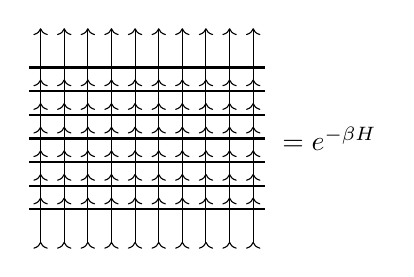
\begin{tikzpicture}[xscale=1.5,decoration={
    markings,
    mark=at position 0.5 with {\arrow{>}}}]

    
    \foreach \i in {0.1,0.3,...,1.9} {
        \draw[->] (\i, 1.8) -- (\i, 2.3);
        \draw[-<] (\i, 0) -- (\i, -0.5);
    }
    \foreach \i in {0,0.3,...,2.1} {
        \draw[thick] (0, \i) -- (2, \i);
    }
    \foreach \i in {0,0.3,...,1.8} {
        \foreach \j in {0.1,0.3,...,1.9} {
            \draw[postaction={decorate}] (\j, \i) -- ++(0, 0.3);
        }
    }
    \draw (2, 0.9) node[anchor=west] {${}= e^{-\beta H}$};
\end{tikzpicture}
\end{document}